\chapter{Công nhệ NodeJS}
\section{Mô hình WebServer truyền thống}
    Trước hết ta tìm hiểu hoạt động của server.  Server truyền thống hoạt động theo cơ chế \texttt{synchronize IO}. Khi client gửi đến server một yêu cầu, server sẽ dựa trên url yêu cầu để tìm tài nguyên tương ứng. Server sẽ đợi vào ra dữ liệu.Tùy vào tài nguyên đó, server có thể gọi một chương trình khác để tiền xử lý (ví dụ php) và trả lại kết quả cho client. Để đáp ứng được yêu cầu cho nhiều client, server sẽ sử dụng thread để quản lý mỗi yêu cầu của client. Để tăng cường hiệu quả sử dụng thread, các server thường sử dụng cơ chế spool thread. Mô hình này có thể mô hình bởi hình vẽ dưới đây. \\
	\begin{figure}
        \centering
        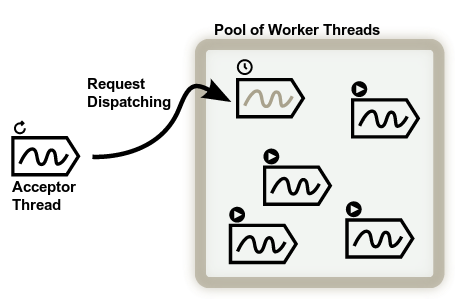
\includegraphics[scale=0.7]{io}
        \rule{35em}{0.5pt}
        \caption{Mô hình Server truyền thống}
        \label{fig:io}
    \end{figure}
	Như có thể thấy trong hình \ref{fig:io}, khi có một yêu cầu được chấp nhận. Bộ phân phối yêu cầu sẽ tìm thread rảnh rỗi và phân phổi yêu cầu cho thread đó.
	Tuy nhiên, mô hình này vẫn chứa những hạn chế nhất định. Đó là: \\
	\begin{itemize}
		\item Hạn chế của  việc sử dụng luồng: Việc sử dụng luồng có nhưng hạn chế nhất định. Trước hết, số lượng luồng tối đa có thể tạo ra bị giới hạn bởi khả năng của CPU. Tiếp đến là chi phí quản lý luồng cực kỳ tốn kém đặc biệt khi số lượng luồng lớn(khởi tạo luồng, lập lịch và chuyển đổi luồng, hủy bỏ luồng).
		\item Lãng phí CPU do thời gian vào ra IO. Khi một yêu cầu từ client gửi tới, server sẽ phải đọc dữ liệu được định danh trong url, và chuyển nó tới bộ tiền xử lý. Trong thời gian vào ra, thread đó hoàn toàn không có tính toán. Do vậy hiệu xuất sử dụng CPU rất thấp.
		\item Việc đồng bộ giữa các thread: Trong trường hợp  muốn đồng bộ giữa các thread, việc này cực kỳ khó.
	\end{itemize}

     \section{NodeJS, mô hình server mới}
	\subsection{Mô hình NodeJS}
	Khác với cơ chế truyền thống, NodeJS hoạt động theo cơ chế \texttt{asynchronous IO}. Trong NodeJS, có duy nhất một tiến trình hoạt động. Khi yêu cầu gửi từ client đến, server sẽ gửi yêu cầu cho bộ phận vào ra về yêu cầu đó và tiếp tục lắng nghe các yêu cầu khác từ client. Khi đã kết thúc vào ra, bộ phận vào ra gửi tín hiệu ngắt tới server. Server sẽ nhận dữ liệu này và tiếp tục xử lý. Như vậy, hiệu xuất sử dụng CPU đã tăng nên. Hơn nữa, trong trường hợp này, do chỉ có một tiến trình duy nhất, ta không còn gặp phải vấn đề về thread và đồng bộ giữa các Thread như trong mô hình cũ gặp phải nữa. Mô hình hoạt động của NodeJS được theer hiện trong hình dưới đây:
	\begin{figure}
        \centering
        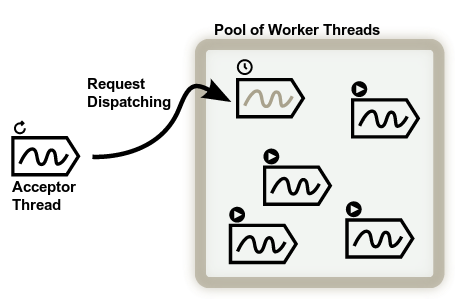
\includegraphics[scale=0.7]{io}
        \rule{35em}{0.5pt}
        \caption{Mô hình hoạt động của NodeJS}
        \label{fig:nio}
    \end{figure}
	Theo cơ chế này, khi có ngắt xuất hiện, server sẽ tiếp tục thực hiện xử lý với dữ liệu được đọc. Vậy làm thế nào server có thể xác định được công việc cần phải làm? Giả sử đây là một công việc cần thực hiện của server:
\begin{minted}{javascript}
	var post = db.query('SELECT * FROM posts where id = 1');

	// processing from this line onward cannot execute

	// until the line above completes

	doSomethingWithPost(post);

	doSomethingElse();
\end{minted}
	Trong ví dụ này server phải thực hiện truy vấn cơ sở dữ liệu. Sau khi thực hiện song truy vấn, ta muốn server thực hiện hàm \texttt{doSomethingWithPost(post)} Trong mô hình \texttt{Asynchronous IO}, làm thế nào để khi truy vấn thực hiện xong, server biết và thực hiện hàm \texttt{ioSomethingWithPost(post)}? NodeJS quản lý theo cơ chế \texttt{Event callback}. \texttt{Event callback} là khái niệm chỉ hàm sẽ được gọi khi có một sự kiện xảy ra.
	Code trên có thể được viết lại như sau:
\begin{minted}{javascript}
	callback = function(post) {
		doSomethingWithPost(post);
	};

	db.query('SELECT * FROM posts where id = 1', callback);
	doSomethingElse();
\end{minted}
	Cách tiếp cận này khá đơn giản và hợp lý. Ta sẽ truyền hàm cần thực thi như một tham số của truy vấn. Khi quá trình IO kết thúc, callback sẽ được gọi.
	Vấn đề còn lại duy nhất là làm sao quản lý ngữ cảnh của hàm. Khi hàm trên được gọi, các biến môi trường đang ở trạng thái nào? Ryan Dahl , tác giả của NodeJS ban đầu viết sử dụng ngôn ngữ C, tuy nhiên do việc quản lý ngữ cảnh giữa các callback rất phức tạp, ông đã chuyển sang dùng ngôn ngữ Lua. Lua có cả các thư viện non IO blocking và I/O blocking có thể gây phức tạp cho các nhà lập trình vì vậ Lua không phải là một giải pháp hay. Sau đó, ông nghĩ tới javascript. Trong javascript, có một đặc trưng thú vị là closure function. Khi một hàm được gọi, trước hết bộ thông dịch sẽ tìm các biến cục bộ của hàm sẽ được tham chiếu. Nếu biến đó không tồn tại, bộ thông dịch tiếp tục tìm kiếm ra toàn cục. Ngữ cảnh của hàm được xác định khi hàm được khai báo. Để hiểu kỹ vấn đề này hơn, ta cùng xem ví dụ đơn giản sau:

\begin{minted}{javascript}
var clickCount = 0;
	
document.getElementById('mybutton').onclick = function() {
	clickCount ++;
}
\end{minted}
	Trong ví dụ này, hàm callback ở đây thực hiện đếm số lần click vào một nút. Biến clickCount ở đây không được khai báo trong hàm. Do vậy nó chính là biến toàn cục. Do tại thời điểm khai báo, biến clickCount đã tồn tại, nên đây chính là biến được tham chiếu đến khi callback được gọi.
	
\subsection{Một kết quả benchmark}
Trong phần này ta cùng làm một ví dụ benchmark đơn giản để so sánh hiệu năng của 2 mô hình \\
	\subsubsection{NodeJs vs Apache PHP benchmark}

Tất cả các bài so sánh đều được thực hiện trong điều kiện:
\begin{framed}
	\begin{itemize}
		\item Server Apache 2.2.22
		\item Apache Bench 2.3
		\item Node.js v0.8.12
		\item Laptop: 
		
		\begin{itemize}
			\item Ubuntu: Release 12.04(precise) 32-bit
			\item KernelLinux 3.2.0-38-generic-pae
			\item GNOME 3.4.2
		\end{itemize}		

		\item Hardware:
		\begin{itemize}
			\item Memory: 3.8 GB
			\item Processor: IntelCore i3-2330M CPU @ 2.20GHz x 4
		\end{itemize}
	\end{itemize}
\end{framed}
	
	Chương trình này có $2$ tùy chọn quan trọng là -n số yêu cầu và -c số lượng yêu cầu đồng thời và cuối cùng là url.\\
Test với Node.js: \\
	\begin{center}
		\fbox{\texttt{/usr/bin/ab -n 100000 -c 1000 http://localhost:8080/}}
	\end{center}

Test với Apache:
	\begin{center}
		\fbox{\texttt{/usr/bin/ab -n 100000 -c 1000 http://localhost/}}
	\end{center}


\subsubsection*{Test với chương trình HelloWorld}
Chương trình đơn giản dùng để test với node.js server và Apache:\\
\texttt{hello.js}
	\begin{framed}
		\inputminted[tabsize=4,linenos=true]{javascript}{hello.js}
	\end{framed}

\texttt{index.php}
	\begin{framed}
		\inputminted[tabsize=4,linenos=true]{php}{index.php}
	\end{framed}

%========== Kết quả test HelloWorld ===============
Sau quá trình test ta thu được các kết quả dưới bảng sau:(Thời gian tính theo đơn vị giây)\\
\textbf{$100,000$ yêu cầu, $1000$ yêu cầu đồng thời} \\
	\begin{tabular}{|c|c|c|c|c|c|}
		\hline
		x & 1 & 2 & 3 & 4 & 5 \\
		\hline
		Apache & 25.972 & 27.908 & 26.708 & 29.893 & 25.980 \\
		\hline
		NodeJs & 14.467 & 14.643 & 15.854 & 16.724 & 14.389
		\\ \hline
	\end{tabular}
\newpage

Đồ thị minh họa:\\
	\begin{figure}[-h]
		\centering
		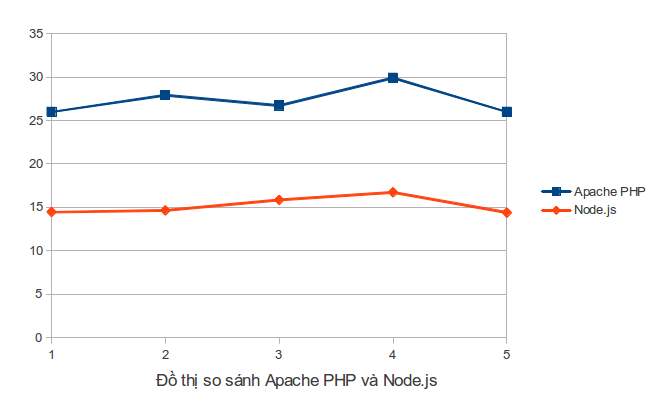
\includegraphics[scale=0.6]{1_1.png}
	\end{figure}

\subsection{Test với chương trình tính số PI}
	Chương trình sử dụng để test:\\
\texttt{testPI.js}
		\begin{framed}
			\inputminted[tabsize=4, linenos=true]{javascript}{testPI.js}
		\end{framed}

\texttt{testPI.php}
		\begin{framed}
			\inputminted[tabsize=4, linenos=true]{php}{testPi.php}
		\end{framed}

%========== Kết quả tính toán số PI ===============
Sau quá trình test ta thu được kết quả trong bảng dưới đây:	\\
	\begin{tabular}{|c|c|c|c|c|c|}
		\hline
		x & 1 & 2 & 3 & 4 & 5 \\
		\hline
		Apache & 26.001 & 27.134 & 26.801 & 28.201 & 27.040 \\
		\hline
		NodeJs & 3.181 & 3.198 & 3.423 & 4.214 & 3.426
		\\ \hline
	\end{tabular}


Đồ thị minh họa:\\
	\begin{figure}[-h]
		\centering
		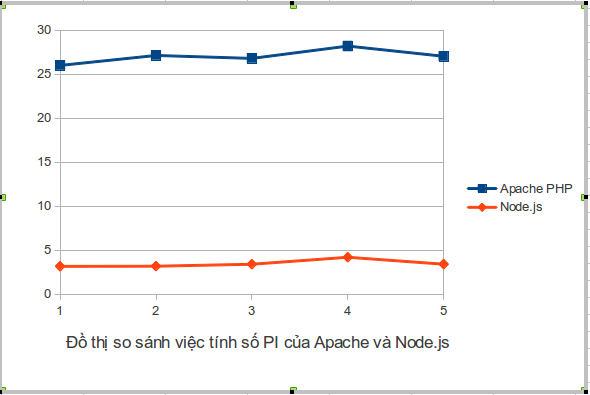
\includegraphics[scale=0.6]{1_2.png}
	\end{figure}


\subsection{Lập trình hướng sự kiện trên server}
	Với việc ra đời NodeJS, cũng dẫn đến một mô hình lập trình mới trên server. Đó là lập trình hướng sự kiện. Phía client, khái niệm này có thể không quá mới mẻ. Trong ngôn ngữ javascript, việc lập trình gắn liền với các sự kiện. Các lập trình viên sẽ tạo các sự kiện DOM và bắt các sự kiện này và sử lý. Với NodeJS, cách lập trình cũng như vậy. Ta cũng bắt các sự kiện từ phía client hoặc các sự kiện từ hệ thống và phản hồi. So với cách lập trình truyền thống, đây là một cách lập trình khá thú vị, mới mẻ.Để hiểu rõ vấn đề này hơn ta sẽ tìm hiểu các module được trình bày trong chương 3 của bài báo
